%% these.tex
%% Copyright 2010 Luca De Feo
%% All rights reserved


The goal of this part of the document is to present some efficient
algorithms to compute in some specific finite dimensional algebras
over a field $\K$.

Let $\K$ be a field, and let $x_1,\ldots,x_n$ be indeterminates. We
denote by $\K[\lst{x}]$ the algebra $\K[x_1,\ldots,x_n]$. Any finite
dimensional $\K$-algebra $\algeb{A}$ is isomorphic to a quotient
$\K[\lst{x}]/I$ for some $0$-dimensional ideal $I$. Residue classes of
$\K[\lst{x}]$ modulo an ideal $I$ are indeed a very good
representation of the elements of $\algeb{A}$.

The most popular tools to compute in generic residue class rings are
Gröbner
bases~\cite{buchberger,cox+little+oshea,Cox-Little-OShea:UAG2005,faugere99,faugere02}.
An alternative to Gröbner bases, called \emph{geometric resolution} is
presented in~\cite{giusti+lecerf+salvy01}. In the bivariate case,
resultants~\cite{cox+little+oshea,Cox-Little-OShea:UAG2005} are a
classic tool.

Besides the algorithmic tool used to compute in $\algeb{A}$, the
choice of a basis for the ideal $I$ also has a great impact. Consider,
for example, the ideal of $\Q[x,y]$
\begin{equation}
  \label{eq:example-x<y}
  (x^2 + x + 1, y^3 - x)
  \text{,}
\end{equation}
another set of generators for the same ideal is
\begin{equation}
  \label{eq:example-y<x}
  (y^6 + y^3 + 1, x - y^3)
  \text{.}
\end{equation}
Both sets of generators are Gröbner bases of $I$ and identify
$\Q[x,y]/I$ to $\Q(\zeta_9)$. However, while \eqref{eq:example-x<y}
naturally identifies $\Q[x]/(x^2+x+1)$ to the subfield
$\Q(\zeta_3)\subset\Q(\zeta_9)$, this information is lost by
\eqref{eq:example-y<x}, making it harder to test for membership in
$\Q(\zeta_3)$ in this case.

Thus, algorithms to change from a set of generators to another are
important too. The FGLM algorithm~\cite{FGLM} computes the change from
a Gröbner basis to another. There is also a variety of change-of-order
algorithms for triangular sets based on
resultants~\cite{boulier+lemaire+moreno01}, on trace
formulas~\cite{diaz+gonzalez01,pascal+schost06}, on Newton-Hensel
lifting~\cite{dahan+jin+moreno+schost08}; while the \emph{rational
  univariate representation} algorithm~\cite{rouiller99} allows to go
from a Gröbner basis to a geometric resolution.

In this chapter we focus on a generalization of
\hyperref[sec:chin-rema-algor]{Lagrange interpolation formula}, called
\emph{trace formulas}, and on its application to the rational
univariate representation of a zero-dimensional
ideal. Section~\ref{sec:decomp-zero-dimens} studies the decomposition
of a zero dimensional ideal in the algebraic closure of $\K$, then
Section~\ref{sec:dual} introduces the trace formulas, and, in
Section~\ref{sec:multiplication}, Stickelberger's theorem makes the
link between the trace formulas and the trace of the multiplication
operator. We present the rational univariate representation algorithm
and some algorithmic improvements in
Sections~\ref{sec:rati-univ-repr},~\ref{sec:univariate-case}
and~\ref{sec:shoups-algorithm}; finally, in
Section~\ref{sec:from-univ-bivar} we show how it can be applied as a
change-of-basis algorithm.


\section{Decomposition of a zero-dimensional ideal}
\label{sec:decomp-zero-dimens}

We let $I$ be a zero-dimensional ideal of $\K[\lst{x}]$ and
$\algeb{A}=\K[\lst{x}]/I$.  To simplify the exposition, from now on we
assume that $\K$ is a perfect field and $I$ is radical, this is
equivalent to all the points of $V(I)=\{a\in\clot{\K}^n|f(a)=0,
\forall f\in I\}$ being simple. We address the reader interested in
the case of arbitrary multiplicity to~\cite{mourrain+elkadi}.

\pdfmcone{Changed "variety" to "algebraic set" for consistency.}
To better understand the structure of $\algeb{A}$ it will be important
to study the algebraic set $V(I)$. We denote by $\clot{I}$ the ideal of
$\clot{\K}[\lst{x}]$ generated by $I$ and by $\clot{\algeb{A}}$ the
quotient ring $\clot{\K}[\lst{x}]/\clot{I}$.

\begin{lemma}
  $\algeb{A}$ is naturally identified to a subset of $\clot{\algeb{A}}$.
\end{lemma}
\begin{proof}
  We want to prove $\clot{I}\cap\K[\lst{x}]=I$. The direction
  $\supset$ is clear. Let $f\in\clot{I}\cap\K[x]$ and let
  $f_1,\ldots,f_k$ be generators of $I$, then there exist
  $g_1,\ldots,g_k\in\clot{\K}[\lst{x}]$ such that
  \begin{equation}
    \label{eq:114}
    f = \sum_i g_if_i
    \text{.}
  \end{equation}
  Then the coefficients of $g_1,\ldots,g_k$ are the solutions of a
  linear system with coefficients in $\K$, thus they can be taken in
  $\K[\lst{x}]$.

  Hence $f\equiv f'\bmod I$ if and only if $f\equiv f'\bmod\clot{I}$.
\end{proof}

Because of the lemma, we will always implicitly identify elements of
$\algeb{A}$ to their image in $\clot{\algeb{A}}$.

\begin{lemma}
  The dimension of $\clot{\algeb{A}}$ as $\clot{\K}$-vector space is
  the same as the dimension of $\algeb{A}$ as $\K$-vector space.
\end{lemma}
\begin{proof}
  Observe that $\clot{\algeb{A}}$ is generated as $\clot{\K}$-vector
  space by the monomials $M=\{\lst{x}^\alpha|\alpha\in\N^n\}$. Since
  $M\subset\algeb{A}$, any generating family of $\algeb{A}$ as
  $\K$-vector space also generates $\clot{\algeb{A}}$ as
  $\clot{\K}$-vector space.  Now, if $a_0,\ldots,a_d$ are
  $\K$-linearly dependent elements of $\algeb{A}$, they clearly are
  $\clot{\K}$-linearly dependent in $\clot{\algeb{A}}$. Thus the
  dimension of $\clot{\algeb{A}}$ does not exceed the one of $\algeb{A}$.

  Now suppose that $\clot{\algeb{A}}$ has dimension $d$ and let
  $a_0,\ldots,a_d$ be elements of $\algeb{A}$. Then, if
  $f_1,\ldots,f_k$ are generators of $I$, there exist
  $\lambda_0,\ldots,\lambda_d\in\clot{\K}$ and
  $g_1,\ldots,g_k\in\clot{\K}[\lst{x}]$ such that
  \begin{equation}
    \label{eq:115}
    \sum_i \lambda_ia_i = \sum_j g_jf_j
    \text{.}
  \end{equation}
  As in the proof of the previous lemma, $\lambda_0,\ldots,\lambda_d$
  and the coefficients of $g_1,\ldots,g_k$ are the solutions of a
  linear system with coefficient in $\K$, thus they can be taken in
  $\K$. Hence $a_0,\ldots,a_d$ are $\K$-linearly dependent.
\end{proof}


In what follows, we suppose that $V(I)$ has cardinality $d$ and we
denote its points by $\zeta_i\in\clot{\K}^n$ for $1\le i\le d$.

\begin{proposition}
  The number of points of $V(I)$ equals the dimension of
  $\clot{\algeb{A}}$ as vector space.
\end{proposition}
\begin{proof}
  Since $\clot{I}$ is radical and zero-dimensional, its primary
  decomposition is
  \begin{equation}
    \label{eq:1}
    \clot{I}=Q_1\cap \cdots \cap Q_d
    \text{,}
  \end{equation}
  where $Q_i$ is the ideal vanishing on $\zeta_i$.
  
  The $Q_i$'s are maximal and pairwise coprime (i.e.\
  $Q_i+Q_j=\clot{\K}[\lst{x}]$ whenever $i\ne j$), hence, by the
  \titleref{th:chinese-remainder},
  \begin{equation}
    \label{eq:3}
    \clot{\K}[\lst{x}]/Q_1\cap\cdots\cap Q_d \isom \bigoplus_{i=1}^d\clot{\K}[\lst{x}]/Q_i
    \text{.}
  \end{equation}

  But $Q_i$ is maximal, hence $\clot{\K}[\lst{x}]/Q_i$ is an algebraic
  field extension of $\clot{\K}$. Since $\clot{\K}$ is algebraically
  closed, $\clot{\K}[\lst{x}]/Q_i=\clot{\K}$, and $\clot{\algeb{A}}$ has
  dimension $d$ as expected.
\end{proof}


\begin{example}
  \begin{figure}[ht]
    \centering
    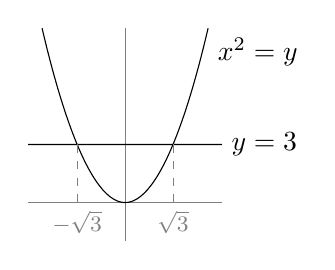
\begin{tikzpicture}
      \draw[x=10pt,y=7pt,gray,very thin]
      (-3.5,0) -- (3.5,0)
      (0,9) -- (0,-2);
      \draw[x=10pt,y=7pt]
      (-3,9) parabola bend (0,0) (3,9) node[anchor=north west]{$x^2=y$}
      (-3.5,3) -- (3.5,3) node[anchor=west]{$y=3$};
      \footnotesize
      \draw[x=10pt,y=7pt,gray,very thin,dashed]
      (-1.73205080756887729352,3) -- (-1.73205080756887729352,0)
      node[anchor=north]{$-\sqrt{3}$}
      (1.73205080756887729353,3) -- (1.73205080756887729353,0)
      node[anchor=north]{$\sqrt{3}$};
    \end{tikzpicture}
    \caption{Plot in the reals of the ideal $I=(y-3,x^2-y)$.}
    \label{fig:ideal-parabola-line}
  \end{figure}

  \pdfmcone{Changed "variety" to "set of zeros" or "algebraic
    set", for consistency with the first part.}  Consider the ideal
  $I=(y-3,x^2-y)$ of $\Q[x,y]$, a plot is given in
  Figure~\ref{fig:ideal-parabola-line}. This ideal is prime and its
  set of zeros contains no $\Q$-rational points. Since
  $G=\{y-3,x^2-y\}$ is a Gröbner basis for $I$ (for grevlex), elements
  of $\algeb{A}=\Q[x,y]/I$ are uniquely represented by their normal
  form modulo $G$; for example
  \[x^5y + 3xy + 1 \equiv 36x + 1 \mod I\text{.}\] By analyzing the
  leading monomials of $G$, it is straightforward to realize that all
  normal forms modulo $G$ have degree at most $1$ in $x$ and degree
  $0$ in $y$, thus $\algeb{A}$ has dimension $2$ as vector space.

  Indeed, the algebraic set $V(I)$ consists of two points:
  \[V(I)=\left\{(\sqrt{3},3), (-\sqrt{3},3)\right\}\subset\clot{\Q}^2\text{.}\]
  Hence, $\clot{I}=(x-\sqrt{3},y-3)\cap(x+\sqrt{3},y-3)$ and
  \[\clot{\algeb{A}}\isom \clot{\Q}/(x-\sqrt{3},y-3) \oplus
  \clot{\Q}/(x+\sqrt{3},y-3)\text{.}\] In particular, the element
  $36x+1$ of $\clot{\algeb{A}}$ is mapped to
  \[(1+36\sqrt{3},1-36\sqrt{3})\] by this isomorphism. The reader will
  have noticed that $\algeb{A}$ is isomorphic to $\Q(\sqrt{3})$ as a ring.
\end{example}

We set 
\begin{equation}
  \label{eq:4}
  \clot{\algeb{A}}_i\eqdef \clot{\K}[\lst{x}]/Q_i
  \text{,}
\end{equation}
then by Eq. \eqref{eq:3} 
\begin{equation}
  \label{eq:5}
  \clot{\algeb{A}} = \bigoplus_{i=1}^d\clot{\algeb{A}_i}
  \text{.}
\end{equation}

Now, the $\clot{\algeb{A}}_i$'s are subalgebras of $\clot{\algeb{A}}$
isomorphic to $\clot{\K}$. We denote by $\basis{e}_i$ the unit element
of $\clot{\algeb{A}}_i$, then
\begin{equation}
  \label{eq:6}
  \begin{aligned}
    \basis{e}_i^2 &= \basis{e}_i\text{,}\\
    \basis{e}_i\basis{e}_j &= 0\text{.}
  \end{aligned}
\end{equation}
Hence $(\basis{e}_1,\ldots,\basis{e}_d)$ is a basis of
$\clot{\algeb{A}}$ made of orthogonal idempotents.

\begin{example}
  \label{ex:trace}
  Continuing the previous example, 
  \[\clot{\algeb{A}}_1 = \clot{\Q}/(x-\sqrt{3},y-3)
  \quad\text{and}\quad
  \clot{\algeb{A}}_2 = \clot{\Q}/(x+\sqrt{3},y-3)
  \text{.}\]
  The idempotents are given by
  \[\basis{e}_1 = (3+\sqrt{3}x)/6
  \quad\text{and}\quad \basis{e}_2 = (3-\sqrt{3}x)/6 \text{.}\] The
  verification of Eq. \eqref{eq:6} is straightforward. In particular
  \[36x + 1 = (1+36\sqrt{3})\basis{e}_1 + (1-36\sqrt{3})\basis{e}_2
  \text{.}\]
\end{example}

For any $f\in\clot{\K}[\lst{x}]$, we denote by $f(\zeta_i)$ the
evaluation of $f$ at $\zeta_i\in V(I)$. $f(\zeta_i)$ only depends on
the class of $f$ in $\algeb{\clot{A}}$, thus for
$a\in\clot{\algeb{A}}$, we define $a(\zeta_i)$ as the evaluation at
$\zeta_i$ of an arbitrary representative of the class $a$.

For any $a\in\clot{\algeb{A}}$, its class in $\clot{\algeb{A}}_i$ is $a(\zeta_i)$,
by Eq. \eqref{eq:4}. Hence
\begin{equation}
  \label{eq:2}
  a = \sum_{i=1}^da(\zeta_i)\basis{e}_i
  \text{.}
\end{equation}

The basis $(\basis{e}_1,\ldots,\basis{e}_d)$ is a very practical one
to represent elements of $\clot{\algeb{A}}$. Unfortunately, in the
general case the idempotents $\basis{e}_i$ may not be elements of
$\algeb{A}$, as the previous example shows; thus, using such a basis
comes at the cost of lifting coefficients in $\clot{\K}$. In order to
find a basis better suited to represent elements of $\algeb{A}$, we
shall study the dual of the algebra $\clot{\algeb{A}}$.


\section{Trace formulas}
\label{sec:dual}
We shall denote by $\dual{\algeb{A}}$ the dual space of $\algeb{A}$,
that is the space of $\K$-linear forms on $\algeb{A}$. Similarly, we
shall denote by $\dual{\clot{\algeb{A}}}$ the dual space of
$\clot{\algeb{A}}$.

The map
\begin{equation}
  \label{eq:8}
  \begin{aligned}
  \basis{1}_{\zeta_i} : \clot{\algeb{A}} &\ra \clot{\K}\\
  a &\mapsto a(\zeta_i)
  \end{aligned}
\end{equation}
is linear; in particular
\begin{equation}
  \label{eq:9}
  \basis{1}_{\zeta_i}(\basis{e}_j) =
  \begin{cases}
    1 &\text{if $i=j$,}\\
    0 &\text{if $i\ne j$.}
  \end{cases}
\end{equation}
Hence $(\basis{1}_{\zeta_1},\ldots,\basis{1}_{\zeta_d})$ is the basis
of $\dual{\clot{\algeb{A}}}$ dual to $(\basis{e}_1,\ldots,\basis{e}_d)$.

\pdfmcone{I don't think it is interesting to recall the
  transposed multiplication here: I already do it in Section 6 (right
  after lemma 19), where the algorithmic content of the formulas is
  discussed.} The space $\dual{\algeb{A}}$ has a natural
$\algeb{A}$-module structure under the law
$\cdot:\algeb{A}\times\dual{\algeb{A}}\ra\dual{\algeb{A}}$ defined by
\begin{equation}
  \label{eq:10}
  \begin{aligned}
    a\cdot\ell : \algeb{A} &\ra \K\\
    b &\mapsto \ell(ab)
    \text{.}
  \end{aligned}
\end{equation}
Similarly $\dual{\clot{\algeb{A}}}$ has an $\clot{\algeb{A}}$-module
structure under an analogous law.

\begin{proposition}
  \label{th:gorenstein}
  $\dual{\clot{\algeb{A}}}$ and $\clot{\algeb{A}}$ are isomorphic as
  $\clot{\algeb{A}}$-modules under the mapping
  $\rho:\basis{e}_i\mapsto\basis{1}_{\zeta_i}$ for $1\le i\le d$.
\end{proposition}
\begin{proof}
  The mapping is clearly a vector space isomorphism, we only need to
  prove that it is a morphism of $\clot{\algeb{A}}$-modules. We want
  to prove that for any $a,b\in\clot{\algeb{A}}$
  \[\rho(ab) = a\cdot\rho(b)\text{.}\]
  It suffices to prove this on the bases
  $(\basis{e}_1,\ldots,\basis{e}_d)$ and
  $(\basis{1}_{\zeta_1},\ldots,\basis{1}_{\zeta_i})$.

  On the one hand
  \begin{equation}
    \label{eq:12}
    \rho(\basis{e}_i\basis{e}_j)=
    \begin{cases}
      \rho(0)=0 &\text{if $i\ne j$,}\\
      \rho(\basis{e}_i)=\basis{1}_{\zeta_i} &\text{if $i=j$.}
    \end{cases}
  \end{equation}
  On the other hand, $\basis{e_i}\cdot\basis{1_{\zeta_j}}$ is the form
  that associates to any $c\in\clot{\algeb{A}}$ the element
  \begin{equation}
    \label{eq:13}
    (\basis{e_i}c)(\zeta_j) = \basis{e}_i(\zeta_j)c(\zeta_j) = 
    \begin{cases}
      0 &\text{if $i\ne j$,}\\
      c(\zeta_j) &\text{if $i=j$,}
    \end{cases}
  \end{equation}
  where the last equality comes from \eqref{eq:9}. Hence
  \begin{equation}
    \label{eq:14}
    \basis{e}_i\cdot\basis{1}_{\zeta_j}=
    \begin{cases}
      0 &\text{if $i\ne j$,}\\
      \basis{1}_{\zeta_i} &\text{if $i=j$.}
    \end{cases}
  \end{equation}
\end{proof}

\begin{nota}
  We have thus identified $\dual{\clot{\algeb{A}}}$ to
  $\clot{\algeb{A}}$ as $\clot{\algeb{A}}$-modules, this implies that
  $\clot{\algeb{A}}$ is a Gorenstein algebra~\cite[Chapter
  8]{mourrain+elkadi}. The theory of Gorenstein algebras is much
  deeper than the exposition we give here, and giving a complete
  account of it would be beyond the scope of this
  document. Nevertheless, we will eventually point out the
  relationships between the results proven here and the general
  theory.
\end{nota}

Since $1$ generates $\clot{\algeb{A}}$ as an $\clot{\algeb{A}}$-module, the form
\begin{equation}
  \label{eq:7}
  \Tr \eqdef \rho(1) = \sum_i\basis{1}_{\zeta_i}
\end{equation}
generates $\dual{\clot{\algeb{A}}}$ as an $\clot{\algeb{A}}$-module.
$\rho(1)$ will play an important role in the sequel; it is called the
\emph{trace form}, the reason for this will be clear in the next
section.

The bilinear form on $\dual{\clot{\algeb{A}}}\times\clot{\algeb{A}}$
defined by
\begin{equation}
  \label{eq:11}
  \braket{\ell}{a} = \ell(a)
\end{equation}
is non-degenerate by definition (see Section
\ref{sec:linear-algebra:duality}). By means of the isomorphism $\rho$,
we can transport this to a bilinear form on
$\clot{\algeb{A}}\times\clot{\algeb{A}}$: we define
\begin{equation}
  \label{eq:15}
  \braket{a}{b}=\rho(a)(b)
  \text{.}
\end{equation}
By Proposition \ref{th:gorenstein}, by Eq. \eqref{eq:10} and by the
equality
\begin{equation}
  \label{eq:16}
  \rho(a)(b) = \sum_i a(\zeta_i)b(\zeta_i)
  \text{,}
\end{equation}
we deduce that
\begin{equation}
  \label{eq:17}
  \braket{a}{b} = \rho(a)(b) = ab\cdot\Tr(1) = a\cdot\Tr(b) = \Tr(ab) = \braket{b}{a}
  \text{.}
\end{equation}
is a non-degenerate form on $\clot{\algeb{A}}\times\clot{\algeb{A}}$
that identifies $\clot{\algeb{A}}$ to its dual.

In particular, from Eqs.~\eqref{eq:17} and~\eqref{eq:2} we deduce the
\emph{trace formulas} or \emph{interpolation formulas}:
\begin{equation}
  \label{eq:21}
  a = \sum_{i=1}^d\braket{a}{\basis{e}_i}\basis{e}_i=\sum_{i=1}^da(\zeta_i)\basis{e}_i=\sum_{i=1}^da\basis{e_i}
\end{equation}

\begin{nota}
  In the Gorenstein setting, the forms $\basis{1}_{\zeta_i}$ are
  called the \emph{local residues} at $\zeta_i$ and the form
  $\sum\basis{1}_{\zeta_i}$ is called a \emph{global residue}. The
  non-degeneracy of the global residue implies the
  $\clot{\algeb{A}}$-isomorphism between $\clot{\algeb{A}}$ and
  $\dual{\clot{\algeb{A}}}$.  The name ``residue'' comes from complex
  analysis, because in $\C[\lst{x}]/I$ this concept coincides with the
  classical analytic
  residue. See~\cite{bykov+kytmanov+lazman,mourrain+elkadi}.
\end{nota}


\section{Sitckelberger's theorem}
\label{sec:multiplication}

Let $a\in\clot{\algeb{A}}$ and consider the linear map
\begin{equation}
  \label{eq:18}
  M_a:a \mapsto ab
  \text{.}
\end{equation}

\begin{theorem}[Stickelberger]
  \label{th:stickelberger}
  The element $\basis{e_i}$ is an eigenvector of $M_a$ associated to
  the eigenvalue $a(\zeta_i)$. The characteristic polynomial of $M_a$
  is
  \[\prod_{i=1}^d(X-a(\zeta_i))\text{.}\]
\end{theorem}
\begin{proof}
  Using Eqs.~\eqref{eq:21} and~\eqref{eq:6}, we have
  \begin{equation}
    \label{eq:19}
    M_a(\basis{e}_i) = a\basis{e}_i = \braket{a}{\basis{e}_i}\basis{e}_i=a(\zeta_i)\basis{e}_i
    \text{.}
  \end{equation}

  Since the $\basis{e}_i$'s form a basis of $\clot{\algeb{A}}$ as a
  vector space, $M_a$ is diagonalizable and its eigenvalues are the
  $a(\zeta_i)$'s, each counted once.
\end{proof}

\pdfmcone{Link with part I.}  We define the \emph{trace} and
the \emph{norm} of an element of $\clot{\algeb{A}}$ in the same way as
they are \hyperref[sec:basic-galois-theory:galois-extensions]{defined}
for elements of extension fields.

\begin{definition}[Trace, norm]
  \label{def:trace}
  We define the \index{trace}\emph{trace} of $a$ as
  \[\Tr(a) = \Tr(M_a)\]
  and its \index{norm}\emph{norm} as
  \[\Norm(a) = \det(M_a)\text{.}\]
\end{definition}
Then, the following corollary is easily derived.

\begin{corollary}
  \label{th:stickelberger-trace-det}
  One has
  \begin{align}
    \label{eq:23}
    \Tr(a) &= \sum_{i=1}^da(\zeta_i)\\
    \label{eq:24}
    \Norm(a) &= \prod_{i=1}^da(\zeta_i)
  \end{align}
\end{corollary}

By Eqs.~\eqref{eq:23} and~\eqref{eq:7}, it is clear that
$\Tr(a)=\rho(1)(a)$, which justifies the notation we employed in the
last section. 

\begin{theorem}
  $\dual{\algeb{A}}$ is isomorphic to $\algeb{A}$ as
  $\algeb{A}$-module under the restriction of $\rho$ to $\algeb{A}$.
\end{theorem}
\begin{proof}
  When $a,b\in\algeb{A}$, the characteristic polynomial of $M_{ab}$
  has coefficients in $\K$. Thus $\braket{a}{b}=\Tr(ab)$ is in $\K$,
  and the restriction of $\rho(a)$ to $\algeb{A}$ is in
  $\dual{\algeb{A}}$.

  Consider now the quadratic form on $\clot{\algeb{A}}$
  \begin{equation}
    \label{eq:113}
    q(a) = \Tr(a^2)
    \text{.}
  \end{equation}
  Its matrix in the basis $(\basis{e}_1,\ldots,\basis{e}_d)$ is the
  identity matrix, thus it has rank $d$. Now let
  $\basis{B}=(\basis{b}_1,\ldots,\basis{b}_d)$ be a basis of
  $\algeb{A}$, then it is a basis of $\clot{\algeb{A}}$ too. The
  matrix of $q$ on $\basis{B}$ has coefficients in $\K$ and rank $d$,
  thus it also is the matrix of the restriction of $q$ to $\algeb{A}$.

  Hence, $q$ is non degenerate on $\algeb{A}$, and so is
  $\braket{a}{b}$. We deduce that $a\in\algeb{A}$ equals $0$ if and
  only if $\rho(a)\in\dual{\algeb{A}}$ equals $0$. To conclude it
  suffices to observe that $\dual{\algeb{A}}$ and $\algeb{A}$ have the
  same dimension as $\K$-vector spaces.
\end{proof}


\section{Rational Univariate Representation}
\label{sec:rati-univ-repr}
\pdfmcone{Eliminated redundant "variety".}  In many circumstances it
is useful to switch from a multivariate representation of the elements
of $\algeb{A}$ to an univariate one. A \emph{rational univariate
  representation} (RUR)~\cite{rouiller99}, sometimes also called
\emph{geometric resolution}~\cite{giusti+lecerf+salvy01}, of
$\K[x_1,\ldots,x_n]/I$ consists in expressing $V(I)$ as the solution
of the system
\begin{equation}
  \label{eq:22}
  \begin{aligned}
    f(t) &= 0\text{,}\\
    x_1 &= \frac{g_1(t)}{g(t)}\text{,}\\
    &\vdots\\
    x_n &= \frac{g_n(t)}{g(t)}\text{,}    
  \end{aligned}
\end{equation}
where $t$ is a new variable and $f,g,g_1,\ldots,g_n$ are univariate
polynomials with coefficients in $\K$.


\begin{lemma}
  \label{th:multi-newton-sums}
  Let $t\in\algeb{A}$ and let $Q$ be its characteristic
  polynomial. Let $T$ be a fresh variable, then
  \begin{equation}
    \label{eq:25}
    \sum_{i\ge0} \frac{\braket{1}{t^{i}}}{T^{i+1}} = \frac{Q'(T)}{Q(T)}
    \text{.}
  \end{equation}
\end{lemma}
\begin{proof}
  By the trace formulas~\eqref{eq:21}
  \begin{equation}
    \label{eq:26}
    t^i = \sum_{j=1}^d\braket{t^i}{\basis{e}_j}\basis{e}_j
    \text{,}
  \end{equation}
  hence
  \begin{equation}
    \label{eq:27}
    \sum_{i\ge0}\frac{\braket{1}{t^i}}{T^{i+1}} =
    \sum_{i\ge0}\sum_{j=1}^d\frac{\braket{1}{\basis{e}_j}\braket{t^i}{\basis{e}_j}}{T^{i+1}} =
    \sum_{i\ge0}\sum_{j=1}^d\frac{t(\zeta_j)^i}{T^{i+1}}
    \text{.}
  \end{equation}
  Swapping the sums, this equals
  \begin{equation}
    \label{eq:28}
    \sum_{j=1}^d\frac{1}{T-t(\zeta_j)} =
    \frac{\sum_{j=1}^d\prod_{j'\ne j}(T-t(\zeta_j))}{\prod_{j=1}^d(T-t(\zeta_j))} =
    \frac{Q'(T)}{Q(T)}
    \text{,}
  \end{equation}
  where the last equality comes from Theorem \ref{th:stickelberger}.
\end{proof}

\begin{remark}
  \label{rk:newton-sums}
  \pdfmcone{Added details on the characteristic of K.}
  If $\K$ has characteristic $0$, the polynomial $Q$ can be recovered
  from its logarithmic derivative via the formula
  \begin{equation}
    \label{eq:30}
    Q = \exp\left(\int \frac{Q'}{Q}\right)
    \text{.}
  \end{equation}
  

  When the degree $d$ is known in advance, this suggests an efficient
  algorithm to compute $Q$, provided the characteristic of $\K$ is $0$
  or larger than $d$.

  We know that $\Tr(1)=d$, hence 
  \begin{equation}
    \label{eq:32}
    \frac{Q'}{Q} =
    \frac{d}{T} + \sum_{i\ge 1}\frac{\braket{1}{t^i}}{T^{i+1}} 
    \text{.}
  \end{equation}
  We deduce
  \begin{equation}
    \label{eq:33}
    Q = \exp\left(d\log T + \int\sum_{i\ge1}\frac{\braket{1}{t^i}}{T^{i+1}}\right) =
    T^d\exp\left(-\sum_{i\ge 1}\frac{\braket{1}{t^i}}{iT^i}\right)
    \text{,}
  \end{equation}
  then the power series on the right hand side can be exponentiated
  using a Newton iteration.  But $Q$ is a polynomial of degree $d$,
  hence we can truncate the exponent power series to the order
  $O(T^{-d-1})$.

  In conclusion, it is sufficient to know
  \begin{equation}
    \label{eq:34}
    \Tr(t),\ldots,\Tr(t^d)
  \end{equation}
  in order to compute $Q$.
\end{remark}

\begin{example}
  Continuing Example~\ref{ex:trace}, we want to compute the characteristic
  polynomial of $t=36x+1$. We know that
  \[t=36x + 1 = (1+36\sqrt{3})\basis{e}_1 + (1-36\sqrt{3})\basis{e}_2
  \text{,}\]
  hence its traces are easily computed :
  \begin{align*}
    \Tr(t) &= (1 + 36\sqrt{3}) + (1-36\sqrt{3}) = 2\text{,}\\
    \Tr(t^2) &= (1 + 36\sqrt{3})^2 + (1-36\sqrt{3})^2 = 7778\text{.}
  \end{align*}
  We compute the exponential:
  \begin{multline*}
    \exp\left(-\frac{2}{T}-\frac{3889}{T^2} + O(T^{-3})\right)=\\
    \left(1-\frac{2}{T}+\frac{4}{2!T^2}+O(T^{-3})\right)\left(1-\frac{3889}{T^2}+O(T^{-3})\right)=\\
    \left(1 - \frac{2}{T} - \frac{3887}{T^2} + O(T^{-3})\right)
    \text{,}
  \end{multline*}
  hence the characteristic polynomial is
  \[T^2-2T-3887\text{.}\]
\end{example}

Being able to compute characteristic polynomials is not enough to find
a rational univariate representation. Indeed, the element $t$ may not
generate $\algeb{A}$ as a $\K$-algebra, and thus not every element of
$\algeb{A}$ could be represented as a rational function of $t$. We now
give a criterion to find elements that generate $\algeb{A}$.

\begin{definition}[Separating element]
  An element $t\in\algeb{A}$ is said to be \emph{separating} if for
  any $\zeta,\zeta'\in V(I)$
  \[t(\zeta)\ne0 \qquad\text{and}\qquad \zeta\ne\zeta'\Rightarrow t(\zeta)\ne t(\zeta')\text{.}\]
\end{definition}

Separating elements always exist, provided $\algeb{A}$ is large
enough. We do not give here any proof of this fact because in the
applications we have in mind a separating element is always at hand.

\begin{proposition}
  Let $t$ be a separating element, then $1,t,\ldots,t^{d-1}$ are
  $\clot{\K}$-linearly independent.
\end{proposition}
\begin{proof}
  Let $\sum_{i=0}^{d-1}a_it^i =0$, then the polynomial
  $\sum_{i=0}^{d-1}a_iT^i$ has $d$ roots in $\clot{\K}$, namely
  $t(\zeta_i)$ for $1\le i \le d$, hence it is identically null.
\end{proof}

Thanks to this proposition and to Lemma~\ref{th:multi-newton-sums}, we
have a way to find the first line of the representation in
Eq.~\eqref{eq:22}, provided that we know a separating element $t$. We
now have to express $x_1,\ldots,x_n$ as functions of the roots of the
minimal polynomial of $t$.

\begin{theorem}
  \label{th:rur}
  Let $t$ be a separating element of $\algeb{A}$ and let $Q$ be its
  minimal polynomial. Let $a\in\algeb{A}$ and set
  \begin{equation}
    \label{eq:38}
    A(T) = Q(T)\sum_{i\ge0}\frac{\braket{a}{t^i}}{T^{i+1}}
    \text{.}
  \end{equation}
  Then $A(T)$ is a polynomial of degree less than $d$, and
  \begin{equation}
    \label{eq:39}
    a = \frac{A(t)}{Q'(t)}
    \text{.}
  \end{equation}
\end{theorem}
\begin{proof}
  We develop the series as in the proof of Lemma
  \ref{th:multi-newton-sums}:
  \begin{equation}
    \label{eq:40}
    \sum_{i\ge0}\frac{\braket{a}{t^i}}{T^{i+1}} =
    \sum_{j=1}^da(\zeta_j)\sum_{i\ge0}\frac{t(\zeta_j)^i}{T^{i+1}}=
    \frac{\sum_{j=1}^da(\zeta_j)\prod_{j'\ne j}(T-t(\zeta_j))}{Q(T)}
    \text{.}
  \end{equation}
  Hence $A(T)$ is a polynomial of degree less than $d$.

  Now we use the trace formulas to decompose 
  $A(t)$ and $Q'(t)$:
  \begin{align}
    \label{eq:41}
    \braket{A(t)}{\basis{e}_i} &=
    \sum_{j=1}^d a(\zeta_j)\prod_{j'\ne j}(\braket{t}{\basis{e}_i}-t(\zeta_j)) =
    a(\zeta_i)\prod_{j\ne i}(t(\zeta_i)-t(\zeta_j))
    \text{,}\\
    \braket{Q'(t)}{\basis{e}_i} &=
    \prod_{j\ne i}(t(\zeta_i)-t(\zeta_j))
    \text{.}
  \end{align}
  Because $t$ is separating, $\braket{Q'(t)}{\basis{e}_i}\ne0$ for any
  $i$, hence $Q'(t)$ is a unit of $\algeb{A}$. We deduce that
  \begin{equation}
    \label{eq:42}
    \braket{\frac{A(t)}{Q'(t)}}{\basis{e}_i} = a(\zeta_i)
  \end{equation}
  for any $i$. Hence, by the trace formulas
  \begin{equation}
    \label{eq:43}
    \frac{A(t)}{Q'(t)} = \sum_i\braket{\frac{A(t)}{Q'(t)}}{\basis{e}_i}\basis{e}_i =
    \sum_i a(\zeta_i)\basis{e}_i = a
    \text{.}
  \end{equation}
\end{proof}

By taking $a=x_i$, the theorem can be used to find a rational
univariate representation: it suffices to know
\begin{equation}
  \label{eq:44}
  \Tr(x_i),\Tr(x_it),\ldots,\Tr(x_it^{d-1})
\end{equation}
in order to deduce $g_i(T)$ as in the representation~\eqref{eq:22}.

\begin{example}
  We conclude the previous example. We want to find a parameterization
  of $x$ and $y$ with respect to $t=36x+1$. We already know the
  minimal polynomial of $t$:
  \[Q(T) = T^2-2T-3887\text{,}\]
  thus
  \[Q'(T) = 2T-2\text{.}\]
  Now
  \[x=\sqrt{3}\basis{e}_1 -\sqrt{3}\basis{e}_2 \qquad
  y = 3\basis{e}_1 + 3\basis{e}_2\text{,}\]
  hence 
  \begin{align*}
    \Tr(x) &= 0\text{,} & \Tr(xt) &= 216\text{,}\\
    \Tr(y) &= 6\text{,} & \Tr(yt) &= 6\text{.}
  \end{align*}
  We deduce that
  \[x=\frac{216}{2t-2}\text{,}\qquad
  y=\frac{6t-6}{2t-2}\text{.}\]
\end{example}

\begin{nota}
  Theorem~\ref{th:rur} was introduced
  in~\cite{alonso+becker+roy+wormann}. It was used by
  Rouiller~\cite{rouiller99} to give an explicit algorithm to compute
  a rational univariate representation of an arbitrary
  zero-dimensional ideal. This algorithm requires to have a monomial
  basis for the vector space $\algeb{A}$, thus in practice it computes
  a rational univariate representation starting from a Gröbner basis.

  A completely different approach based on Noether's normalization
  theorem, called geometric resolution~\cite{giusti+lecerf+salvy01},
  gives a Gröbner-basis-free alternative for computing rational
  univariate representations.
\end{nota}


\section{The univariate case}
\label{sec:univariate-case}
In this section we shall see that, in the particular case of ideals of
the univariate polynomial ring $\K[x]$, trace formulas reduce to
\hyperref[sec:chin-rema-algor]{Lagrange interpolation} and
Lemma~\ref{th:multi-newton-sums} reduces to Newton's identities.

Any ideal $I$ of $\K[x]$ is principal. Let $f$ be a monic generator of
$I$ and let $\zeta_1,\ldots,\zeta_d$ be its roots in $\clot{\K}$, then
\begin{equation}
  \label{eq:20}
  \clot{\K}[x]/(f) = \bigoplus_{i=1}^d \clot{K}[x]/(x-\zeta_i)
  \text{.}
\end{equation}
Hence, the orthogonal idempotents are given by
\begin{equation}
  \label{eq:29}
  \basis{e}_i = \prod_{j\ne i}\frac{x-\zeta_j}{\zeta_i-\zeta_j}
  \text{.}
\end{equation}
By definition
\begin{equation}
  \label{eq:31}
  \braket{a}{\basis{e_i}} = a(\zeta_i)
  \text{,}
\end{equation}
hence the trace formulas rewrite
\begin{equation}
  \label{eq:35}
  a = \sum_{i=1}^d a(\zeta_i)\prod_{j\ne i}\frac{x-\zeta_i}{\zeta_i-\zeta_j}
  \text{,}
\end{equation}
which is exactly the formula of Lagrange interpolation (see
Eq.~\eqref{eq:225}).

Now we want to compute the Newton sums of $f$, i.e.\ the values
\begin{equation}
  \label{eq:37}
  p_i = \zeta_1^i + \cdots + \zeta_d^i
  \text{.}
\end{equation}
$x$ is a root of $f$ in $\algeb{A}$ and it clearly separates $V(I)$,
then by Lemma \ref{th:multi-newton-sums}
\begin{equation}
  \pdfmctwo{One more equality.}
  \label{eq:45}
  \frac{f'}{f} = \sum_{i\ge0}\frac{\braket{1}{x^i}}{T^{i+1}} =
  \sum_{i\ge0}\frac{\sum_{j=1}^d\zeta_j^i}{T^{i+1}} =
  \sum_{i\ge0}\frac{p_i}{T^{i+1}}
  \text{.}
\end{equation}
\pdfmcone{Newton's identities do not work in characteristic <
  d (I never had noticed !)}  Hence the Newton sums can be recovered
as coefficients of the power series. Inversely, the coefficients of
$f$ can be computed from its Newton sums using Newton's identities;
notice, however, that it is more efficient to use
Remark~\ref{rk:newton-sums} for this.


\section{Shoup's algorithm}
\label{sec:shoups-algorithm}

We have seen that at the heart of the rational univariate
representation is the computation of the coefficients of the power
series
\begin{equation}
  \label{eq:46}
  \sum_{i\ge0}\frac{\braket{a}{t^i}}{T^{i+1}}
\end{equation}
up to a certain precision. In this section we shall find an efficient
way to compute such truncated series.

Consider the univariate polynomial ring $\K[T]$ and identify its dual
space $\dual{\K[T]}$ to $\K[[1/T]]$ via the bilinear form
\begin{equation}
  \label{eq:47}
  \braket{\alpha}{f} = [\alpha f]_0
  \text{,}
\end{equation}
where $\alpha\in\K[[1/T]]$, $f\in\K[T]$ and $[\beta]_i$ is the
coefficient of $T^i$ in $\beta$. So that
\begin{equation}
  \label{eq:48}
  \braket{\sum_{i\ge0}\frac{\alpha_i}{T^i}}{\sum_{j=0}^nf_jT^j} =
  \sum_{i\ge0}\alpha_if_i
  \text{.}
\end{equation}

For a $t\in\algeb{A}$, consider the  evaluation map at $t$
\begin{equation}
  \label{eq:49}
  \begin{aligned}
    \ev_t : \K[T] &\ra \algeb{A}\text{,}\\
    g &\mapsto g(t)
    \text{.}
  \end{aligned}
\end{equation}

\begin{lemma}
  \label{th:shoup}
  For any $t\in\algeb{A}$, the dual map $\dual{\ev_t}$ with respect to
  the bilinear forms defined in Eqs.~\eqref{eq:15} and~\eqref{eq:49}
  is such that
  \begin{equation}
    \label{eq:50}
    \dual{\ev_t}(a) = \sum_{i\ge0}\frac{\braket{a}{t^i}}{T^{i}}
    \text{.}
  \end{equation}
\end{lemma}
\begin{proof}
  $\ev_t$ and $\dual{\ev_t}$ are clearly linear maps, thus it suffices
  to show the identity on the basis $\{1,T,T^2,\ldots\}$ of $\K[T]$.
  \begin{equation}
    \label{eq:51}
    \braket{a}{\ev_t(T^j)} =
    \braket{a}{t^j} =
    \braket{\sum_{k\ge0}\frac{\braket{a}{t^k}}{T^k}}{T^j} =
    \braket{\dual{\ev_t}(a)}{T^j}
    \text{.}
  \end{equation}
\end{proof}

\pdfmcone{Made more precise what we mean by "algorithm".}
Thus, applying the techniques of Section~\ref{sec:stra-line-progr},
from any \hyperref[def:algebraic-transform]{$\K$-algebraic transform}
to compute $\ev_t$ for a fixed $t$ we can deduce a transform to
compute $\dual{\ev_t}$ that has the same time and space
complexity. Furthermore, from a generic
\hyperref[sec:r-algebr-algor]{$\K$-algebraic algorithm} to evaluate
polynomials in $\K[T]$ at points of $\algeb{A}$, we can deduce an
algorithm to compute $\dual{\ev_t}$ for any $t$, having the same time
complexity and possibly a penalty in space complexity.

However, for a given basis of $\algeb{A}$, it may be difficult to find
the corresponding dual basis with respect to $\braket{}{}$. In order
to give an explicit algorithm, we work with the form
\begin{equation}
  \label{eq:52}
  \braket{\ell}{a} = \ell(a)
\end{equation}
on $\dual{\algeb{A}}\times\algeb{A}$, instead.

\begin{lemma}
  Let $a\in\algeb{A}$ and consider the map $M_a:b\mapsto ab$. The dual
  map $\dual{M_a}$ with respect to the form~\eqref{eq:52} is
  such that
  \begin{equation}
    \label{eq:53}
    \dual{M_a}(\ell) = a\cdot\ell
    \text{.}
  \end{equation}
\end{lemma}
\begin{proof}
  The verification is straightforward:
  \begin{equation}
    \label{eq:54}
    \braket{\ell}{M_a(b)} = \braket{\ell}{ab} = \ell(ab) =
    \braket{a\cdot\ell}{b}
    \text{.}
  \end{equation}
\end{proof}

Hence, using Principle~\ref{th:tellegen-princip}, any multiplication
algorithm for a given basis $\basis{B}$ of $\algeb{A}$ can be
transposed to compute $a\cdot\ell$ given $a$ on $\basis{B}$ and $\ell$
on $\dual{\basis{B}}$. Transposed multiplication is a classic problem,
it can be solved without significant losses in space complexity on
most bases, see Section~\ref{sec:transp-algor}
and~\cite{shoup95,shoup99,bostan+lecerf+schost:tellegen,hanrot+quercia+zimmermann,pascal+schost06}.

We now consider again the dual map of $\ev_t$, this time with respect
to \eqref{eq:52}; we denote it by $\proj_t$ to avoid confusion
with~\eqref{eq:50}.

\begin{lemma}
  \label{th:shoup94}
  For any $t\in\algeb{A}$, the map $\proj_t$ is such that
  \begin{equation}
    \label{eq:55}
    \proj_t(\ell) = \sum_{i\ge0}\frac{\ell(t^i)}{T^{i}}
    \text{.}
  \end{equation}  
\end{lemma}
\begin{proof}
  This is just a consequence of Lemma~\ref{th:shoup}, since there
  exists an $a\in\algeb{A}$ such that $\ell=\rho^{-1}(a)$.
\end{proof}

The problem of computing $\proj_t$ is often known as \emph{power
  projection}. Using again Principle~\ref{th:tellegen-princip}, any
algorithm to evaluate polynomials in $\K[T]$ on $t$ can be transposed
to a power projection algorithm on $t$. We will see some instances of
power projection algorithms later on.

Then, the proof of the following theorem is evident.

\begin{theorem}
  \label{th:power-projection}
  Let $a,t\in\algeb{A}$, let $\Tr\in\dual{\algeb{A}}$ be the trace
  form, then
  \begin{equation}
    \label{eq:56}
    \sum_{i\ge0}\frac{\braket{a}{t^i}}{T^i} = \proj_t\circ\dual{M_a}(\Tr)
    \text{.}
  \end{equation}
\end{theorem}

From it, we can derive an algorithm to compute a rational univariate
representation, provided we know the coordinates of the linear form
$\Tr$.

\begin{algorithm}
  \caption{\alg{RUR}}
  \label{alg:rur}
  \begin{algorithmic}[1]
    \REQUIRE A basis $\basis{B}$ of
      $\algeb{A}$, $a_1,\ldots,a_n\in\algeb{A}^{\basis{B}}$, $t$
    separating, $\Tr\in(\dual{\algeb{A}})^{\dual{\basis{B}}}$.
    \ENSURE A rational univariate representation of $a_1,\ldots,a_n,t$.
    \STATE \label{alg:rur:1}Compute $\frac{Q'}{Q} = \frac{1}{T}\proj_t(\Tr)$;
    \STATE \label{alg:rur:2}Compute $Q = \exp\left(\int \frac{Q'}{Q}\right)$;
    \FORALL{$a_i$}
    \STATE \label{alg:rur:4}Compute $A_i(T)=\frac{Q(T)}{T}\cdot(\proj_t\circ\dual{M_{a_i}}(\Tr)) \bmod T^d$;
    \ENDFOR
    \STATE \label{alg:rur:5}Output $Q(T)$ and $\frac{A_1(T)}{Q'(T)},\ldots,\frac{A_n(T)}{Q'(T)}$.
  \end{algorithmic}
\end{algorithm}

In order to apply this algorithm, prior knowledge of the expression of
$\Tr$ in the basis $\dual{\basis{B}}$, i.e.\ $\{\Tr(b) |
b\in\basis{B}\}$, is needed. When $B$ is a polynomial basis
$\{1,b,\ldots,b^d\}$, and the minimal polynomial of $b$ is known in
advance, this can be obtained using Lemma~\ref{th:multi-newton-sums}.

\begin{remark}
  In the univariate case $\algeb{A}=\K[x]/(f)$, $t\in\algeb{A}$ is
  expressed in the basis $(1,x,\ldots,x^{d-1})$ as a polynomial in $x$
  modulo $f$. Then,
  \[\ev_t(g) = g(t) = g\circ t \bmod f\text{,}\]
  where $g\circ t$ is polynomial composition. The problem of computing
  $g\circ t\bmod f$ for $g,t,f\in\K[x]$ is modular composition; as in
  Section~\ref{sec:asympt-compl}, its complexity is denoted by
  $\ModComp(d)$, where $d=\deg f$. A naive algorithm gives
  $\ModComp(d)\in O(d^2)$.
  
  As we saw in Section~\ref{sec:modular-composition}, the most
  efficient algorithms for modular composition are Brent and
  Kung's~\cite{brent+kung}, having complexity $O(\Mult(d)\sqrt{d} +
  d^{(\omega+1)/2})$, and Kedlaya and
  Umans'~\cite{umans:08,kedlaya+umans08}, having quasi-linear
  complexity. Each of these has a dual algorithm solving power
  projection with the same complexity~\cite{shoup94,kedlaya+umans08},
  thus, at least in the univariate case, power projection can be
  solved in subquadratic time.  Some extensions to the bivariate and
  multivariate case also exist~\cite{shoup99,kedlaya+umans08}.
\end{remark}

\begin{remark}
  \label{rk:shoups-algorithm-1}
  \pdfmcone{Added reference to Kaltofen 2k.}  Algorithm~\ref{alg:rur}
  first appeared in~\cite{bostan+salvy+schost03}, which combined the
  ideas of~\cite{rouiller99}
  and~\cite{shoup94,shoup95,shoup99}. Lemma~\ref{th:shoup94} was first
  used in~\cite{shoup94} to compute minimal polynomials of elements of
  a residue class field $\K[x]/(f)$, based on a transposed modular
  composition algorithm. The method was extended to the bivariate case
  in~\cite{shoup99}. A review of the methods
  of~\cite{shoup94,shoup95,shoup99} can be found
  in~\cite[$\S$6]{Ka2K}.

  In~\cite{shoup94,shoup99}, a generic linear form $\ell$ is taken, so
  that by Theorem \ref{th:rur}
  \[\sum_{i\ge0}\frac{\ell(t^i)}{T^{i+1}}=\frac{A(T)}{Q(T)}\]
  for some $A(T)$. Since $\ell$ is arbitrary, $A(T)$ is \emph{a
    priori} unknown, thus one cannot use Remark~\ref{rk:newton-sums}
  to recover $Q$. Instead, a rational fraction reconstruction
  algorithm (see Section~\ref{sec:eucl-algor-rati}) is used to recover
  both $A(T)$ and $Q(T)$. However, in comparison to
  Remark~\ref{rk:newton-sums}, this requires to compute twice as many
  ``power projections''.
  
  The intuition for the method, and for the name ``power projection'',
  comes from Wiedemann's method to solve sparse linear
  systems~\cite{wiedemann:sparse}. The idea is that the minimal
  polynomial of a black-box matrix $A$ is the same as the one of the
  linear recurrent sequence
  \[1,A,A^2,\ldots\] 
  Then, for any linear form $\ell$, the minimal polynomial of the sequence
  \[\ell(1),\ell(A),\ell(A^2),\ldots\]
  divides the minimal polynomial of $A$. The algorithm takes a random
  form $\ell$ and uses it to ``project'' the first $2d$ powers of $A$
  onto $\K$, then recovers its minimal polynomial using the
  Berlekamp-Massey algorithm~\cite{massey69}. On the equivalence
  between the Berlekamp-Massey algorithm and the rational fraction
  reconstruction, see~\cite{dornstetter87}.
\end{remark}


\section{From univariate to bivariate and back again}
\label{sec:from-univ-bivar}

Algorithm \titleref{alg:rur} can be used as an efficient change of basis
algorithm. Let $\basis{B}$ be any basis for $\algeb{A}$, let $t$ be a
separating element, and let the coordinates of $\Tr$ on
$\dual{\basis{B}}$ be known.

\begin{proposition}
  \label{th:uni-multi-uni}
  Let $\Mult_{\basis{B}}$ be the cost of multiplication in the basis
  $\basis{B}$ and let $\mathsf{E}_\basis{B}$ be the cost of the change of basis from
    \begin{equation}
    \basis{T} = (1,t,\ldots,t^{d-1})
  \end{equation}
  to $\basis{B}$. Then, the cost of the change of basis from
  $\basis{B}$ to $\basis{T}$ is
  \begin{equation}
    \label{eq:75}
    \Mult_{\basis{B}} + \mathsf{E}_{\basis{B}} + O(\Mult(d))
    \text{,}
  \end{equation}
  plus a precomputation cost of
  \begin{equation}
    \label{eq:65}
    \mathsf{E}_{\basis{B}} + O(\Mult(d)\log d)
    \text{,}
  \end{equation}
  where $\Mult(d)$ is the cost of polynomial multiplication, as usual.
\end{proposition}

The algorithm follows immediately from the observation that the change
of basis map from $\basis{T}$ to $\basis{B}$ is the same thing as the
map
\begin{equation}
  \begin{aligned}
    \ev_t : \K[T] &\ra \algeb{A}^{\basis{B}}\text{,}\\
    g &\mapsto g(t)\text{.}
  \end{aligned}
\end{equation}
Then algorithm \titleref{alg:rur} on inputs
$a\in\algeb{A}^{\basis{B}}$ and $\Tr$, outputs the expression of $a$
in the basis $\basis{T}$. We now prove the complexity
estimates~\eqref{eq:75} and~\eqref{eq:65}.

\begin{proof}[Proof of Proposition~\ref{th:uni-multi-uni}]
  By Principle~\ref{th:tellegen-princip}, the call to $\proj_t$ at
  step~\ref{alg:rur:1} of \titleref{alg:rur} has the same cost as
  $\mathsf{E}_{\basis{B}}$. Then the cost of step~\ref{alg:rur:2} is
  $O(\Mult(d))$ using a Newton iteration. Both these steps can be done
  just once, thus they contribute to~\eqref{eq:65}.

  Again by Principle~\ref{th:tellegen-princip}, step~\ref{alg:rur:4}
  costs
  \begin{equation}
    \label{eq:80}
    \Mult_{\basis{B}} + \mathsf{E}_{\basis{B}} + \Mult(d)
    \text{,}
  \end{equation}
  where the first term comes from transposed multiplication, the
  second one from the power projection and the third one from
  multiplication by $Q$.

  Finally, in step~\ref{alg:rur:5} instead of expressing $a$ as a
  rational fraction, we need to invert $Q'$ modulo $Q$ and multiply
  $A$ by the result. The inversion costs $O(\Mult(d)\log d)$ by
  extended GCD, but can be done just once, thus it contributes
  to~\eqref{eq:65}; the multiplication costs $O(\Mult(d))$ by
  polynomial multiplication and Newton inversion.
\end{proof}



% Local Variables:
% mode:flyspell
% ispell-local-dictionary:"american"
% mode:TeX-PDF
% mode:reftex
% TeX-master: "../these"
% End:
